\begin{filecontents}{apsrevcontrol.bib}
  @CONTROL{apsrev41Control,title="0"%,author="48",editor="1",pages="1",year="0"}
\end{filecontents}
\RequirePackage[l2tabu, orthodox]{nag}
\documentclass[aps,english,superscriptaddress,twocolumn,twoside,longbibliography,prl,floatfix]{revtex4-1}%

\usepackage[utf8]{inputenx}% for arXiv use encoding ansinew
%\input{ix-utf8enc.dfu}
\usepackage[OT1]{fontenc}
\usepackage{upquote}
\usepackage{amsfonts}
\usepackage{amssymb}
%\usepackage{amsthm}
\usepackage{amsmath}
\usepackage{graphicx}%
\setcounter{MaxMatrixCols}{30}
%TCIDATA{OutputFilter=latex2.dll}
%TCIDATA{Version=5.50.0.2953}
%TCIDATA{CSTFile=revtex4.cst}
%TCIDATA{Created=Thursday, February 14, 2013 01:09:34}
%TCIDATA{LastRevised=Thursday, February 21, 2013 15:16:22}
%TCIDATA{<META NAME="GraphicsSave" CONTENT="32">}
%TCIDATA{<META NAME="SaveForMode" CONTENT="1">}
%TCIDATA{BibliographyScheme=Manual}
%TCIDATA{<META NAME="DocumentShell" CONTENT="Articles\SW\REVTeX 4">}
%BeginMSIPreambleData
\providecommand{\U}[1]{\protect\rule{.1in}{.1in}}
%EndMSIPreambleData
\newtheorem{theorem}{Theorem}
\newtheorem{acknowledgement}[theorem]{Acknowledgement}
\newtheorem{algorithm}[theorem]{Algorithm}
\newtheorem{axiom}[theorem]{Axiom}
\newtheorem{claim}[theorem]{Claim}
\newtheorem{conclusion}[theorem]{Conclusion}
\newtheorem{condition}[theorem]{Condition}
\newtheorem{conjecture}[theorem]{Conjecture}
\newtheorem{corollary}{Corollary}[theorem]
\newtheorem{criterion}[theorem]{Criterion}
\newtheorem{definition}[theorem]{Definition}
\newtheorem{example}[theorem]{Example}
\newtheorem{exercise}[theorem]{Exercise}
\newtheorem{lemma}[theorem]{Lemma}
\newtheorem{notation}[theorem]{Notation}
\newtheorem{problem}[theorem]{Problem}
\newtheorem{proposition}[theorem]{Proposition}
\newtheorem{remark}[theorem]{Remark}
\newtheorem{solution}[theorem]{Solution}
\newtheorem{summary}[theorem]{Summary}
\newenvironment{proof}[1][Proof]{\noindent\textbf{#1.} }{\ \rule{0.5em}{0.5em}}

% hyperlink stuff
\usepackage[usenames,dvipsnames]{color}
\definecolor{ultramarine}{RGB}{63, 0, 255}
\definecolor{medblue}{RGB}{0, 0, 100}
\definecolor{panblue}{RGB}{0,24,150}
\definecolor{carmine}{RGB}{150, 0, 24}
\usepackage[breaklinks=true]{hyperref}
\hypersetup{colorlinks,
linkcolor=carmine,
citecolor=medblue,
urlcolor=panblue,
anchorcolor=OliveGreen}
%\usepackage{url}


\definecolor{purple}{RGB}{128,0,128}
\newcommand{\purp}[1]{{\color{purple}{#1}\color{black}}}

\usepackage{verbatim} %for comment command
\usepackage{units}% for nicefrac
\newcommand{\half}[1]{\nicefrac{#1}{2}}
\newcommand{\brackets}[1]{\lbrace{#1\rbrace}}
\usepackage{microtype}
\usepackage[capitalise]{cleveref}
\Crefname{eqs}{Eqs.}{Eqs.}
\creflabelformat{eqs}{(#2#1#3)}
\crefrangelabelformat{equation}{(#3#1#4-#5#2#6)}
%\crefmultiformat{equation}{eqs.~(#2#1#3)}{ and~(#2#1#3)}{, (#2#1#3)}{ and~(#2#1#3)}
\Crefmultiformat{equation}{Eqs.~(#2#1#3}{,#2#1#3)}{,#2#1#3}{,#2#1#3)}

\usepackage{mathtools} %for mathclap and prescript and more. Learning to love this package. And DeclarePairDelimeter!
\DeclarePairedDelimiter\ceil{\lceil}{\rceil}
\DeclarePairedDelimiter\floor{\lfloor}{\rfloor}


\begin{document}
%\preprint{ }
%\title{Transitivity of implication and causal structure}
\title{Alternatives to Entropic Inequalities and the Triangle Scenario}
\author{Robert W. Spekkens}
\email{rspekkens@perimeterinstitute.ca}
\affiliation{Perimeter Institute for Theoretical Physics, Waterloo, Ontario, Canada, N2L 2Y5}
\author{Tobias Fritz}
\email{tfritz@perimeterinstitute.ca}
\affiliation{Perimeter Institute for Theoretical Physics, Waterloo, Ontario, Canada, N2L 2Y5}
\author{Elie Wolfe}
\email{ewolfe@perimeterinstitute.ca}
\affiliation{Perimeter Institute for Theoretical Physics, Waterloo, Ontario, Canada, N2L 2Y5}
\date{\today}


\begin{abstract}
Given some hypothesis of causal structure it is desirable to determine the set of probability distributions compatible with the hypothesis. For certain causal structures, such as Bell scenarios, the compatible set corresponds to the convex hull of various deterministic distributions, and admits a necessary and sufficient description in terms of conditional probability linear inequalities. For more general causal structures, however, it is far easier to derive entropic inequalities instead of probabilistic inequalities. Unfortunately there typically exist distributions which are genuinely incompatible with the causal structure but which satisfy all the structure's entropic inequalities. A tight characterization of all distributions which can be explained in terms of classical latent variables is critical in quantum information theory in order to recognize and exploit uniquely quantum distributions. The insufficiency of entropic inequalities, therefore, motivates us to explore alternative means of deriving compatibility tests for general causal structures, ideally directly at the level of probabilities. Uniquely quantum distributions are known to exist in the Triangle scenario; the methods presented herein may assist in isolating the criteria which distinguish quantum from classical distributions in that scenario.
\end{abstract}
\maketitle
%In Ref.~\cite{WoodSpekkens}, the standard proof of Bell's theorem is presented in the language of causal inference.  In particular, the CHSH inequality emerges as a special case of what Pearl calls an ``instrumental inequality''.  Hardy's proof of Bell's theorem is quite different from the standard proof and the following question naturally arises: is there a generic tool for classical causal inference of which the Hardy argument can be considered a special case when applied to the M-shaped causal structure of the Bell experiment?

%To try and answer this question, we apply Hardy-type reasoning to the triangle causal structure, that is, the one with three observed variables, each pair of which have a common cause.  We show that this sort of reasoning does indeed facilitate causal inference in the case of the triangle causal structure, thereby lending some evidence to the notion that this style of argument has the potential to be generalized into a generic tool for classical causal inference.


\section{Introduction}
***needs introduction***


\section{Inferential Compatibility Criteria}
Inspired by Hardy-type proofs on nonlocality~\cite{L.Hardy:PRL:1665,CabelloHardyInequality,LSW} we have developed a method to derive compatibility criteria from causal structures. The method is illustrated by examples.
We follow the convention that upper-case indicates random variables while lower-case indicates some value associated with the random variable. Thus $p(ab|xy\lambda)$ should be understood as ${p(A\mathopen{=}a,B\mathopen{=}b|X\mathopen{=}x,Y\mathopen{=}y,\Lambda\mathopen{=}\lambda)}$. We use lower-case subscripts to indicate conditioning upon a particular value, such that for instance $p(a_x b_y|\lambda)=p(ab|xy\lambda)$. The complement of a value is marked by an empty circle accent, so $\mathring{b}$ means ``anything but $b$", and accordingly $P(\mathring{a}\mathring{b})=P(A\mathopen{\neq}a,B\mathopen{\neq}b)$.

\section{Bell Scenario}
\begin{figure}[b!]
 \center{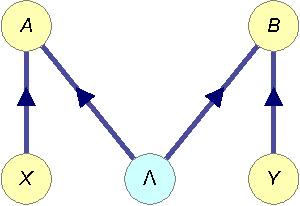
\includegraphics[width=2.0in]{BellDAGcap.pdf}}
\caption{The causal structure of the Bell scenario, on which Bell's theorem is based.}
 \label{fig:BellDAG}
\end{figure}

Consider the causal structure associated to the Bell experiment, depicted in \cref{fig:BellDAG}. 
The assumption of causal structure dictates that
\begin{align}\begin{split}\label{eq:bellstructure}
p(ab|xy\lambda)=p(a_x|\lambda)p(b_y|\lambda)
\end{split}\end{align}
and accordingly that
\begin{align}\begin{split}\label{eq:bellintegration}
&p(a_x b_y)=\sum\limits_{\mathclap{\text{all }\lambda}}p(a_x|\lambda)p(b_y|\lambda)p(\lambda).
\end{split}\end{align}
It is furthermore trivially true that
\begin{align}\begin{split}\label{eq:hardytoproductsums}
&\forall_{y^{\prime}}\!:\quad p(a_x|\lambda)=\sum\limits_{\mathclap{b^{\prime}}}p(a_x|b^{\prime}_{y^{\prime}})p(b^{\prime}_{y^{\prime}}|\lambda),\\
&\forall_{x^{\prime}}\!:\quad p(b_y|\lambda)=\sum\limits_{\mathclap{a^{\prime}}}p(b_y|a^{\prime}_{x^{\prime}})p(a^{\prime}_{x^{\prime}}|\lambda).
\end{split}\end{align}
As such, for any $x^{\prime},y^{\prime}$ we have $p(a_x b_y)=$
\begin{align}\begin{split}
&\sum\limits_{\mathclap{\text{all }\lambda,a^{\prime},b^{\prime}}}p(a_x|b^{\prime}_{y^{\prime}})p(b^{\prime}_{y^{\prime}}|\lambda)p(b_y|a^{\prime}_{x^{\prime}})p(a^{\prime}_{x^{\prime}}|\lambda)p(\lambda).
\end{split}\end{align}
where we can consider specific terms in the sum for convenience, such as one particular $a^{\prime}$ or one particular $b^{\prime}$. In this manner we obtain multiple upper bounds for $p(a_x b_y)$. Formally, $p(a_x b_y)\geq$
\begin{align}\begin{split}\label{eq:doublesums} 
&\forall_{a^{\prime}}\!:\;p(b_y|a^{\prime}_{x^{\prime}})\sum\limits_{\mathclap{\lambda,b^{\prime}}}p(a_x|b^{\prime}_{y^{\prime}})p(b^{\prime}_{y^{\prime}}|\lambda)p(a^{\prime}_{x^{\prime}}|\lambda)p(\lambda),\\
&\forall_{b^{\prime}}\!:\;p(a_x|b^{\prime}_{y^{\prime}})\sum\limits_{\mathclap{\lambda,a^{\prime}}}p(b_y|a^{\prime}_{x^{\prime}})p(b^{\prime}_{y^{\prime}}|\lambda)p(a^{\prime}_{x^{\prime}}|\lambda)p(\lambda).
\end{split}\end{align}
It is possible to evaluate the sums over $\lambda$ in \cref{eq:doublesums} to obtain
\begin{proposition}\label{prop:BellNoGoNEW}The Bell causal structure (\cref{fig:BellDAG}) implies
\begin{align}\begin{split}
&\forall_{x^{\prime},y^{\prime},a^{\prime}}\!:\;p(a_x b_y)\geq p(b_y|a_{x^{\prime}})\sum\limits_{\mathclap{b^{\prime}}}p(a_x|b^{\prime}_{y^{\prime}})p(a^{\prime}_{x^{\prime}}b^{\prime}_{y^{\prime}})\\
&\forall_{x^{\prime},y^{\prime},b^{\prime}}\!:\;p(a_x b_y)\geq p(a_x|b_{y^{\prime}})\sum\limits_{\mathclap{a^{\prime}}}p(b_y|a^{\prime}_{x^{\prime}})p(a^{\prime}_{x^{\prime}}b^{\prime}_{y^{\prime}})
\end{split}\end{align}
\end{proposition}
Of course, Prop.~\ref{prop:BellNoGoNEW} can also be weakened by considering individual terms from the sums. Thus
\begin{corollary}\label{cor:BellNoGoNEW}The Bell causal structure (\cref{fig:TriDAG}) implies% for any ${a^{\prime},b^{\prime},c^{\prime}}$ we have $p(abc)$
\begin{align}\begin{split}
&\forall_{x^{\prime},y^{\prime},a^{\prime},b^{\prime}}\!:\;p(a_x b_y)\geq p(a_x|b_{y^{\prime}})p(b_y|a^{\prime}_{x^{\prime}})p(a^{\prime}_{x^{\prime}}b^{\prime}_{y^{\prime}})
\end{split}\end{align}
\end{corollary}
Consider the following special case, where $p(a_1|b_0)=p(b_1|a_0)=1$. For this case, taking ${a^{\prime}\mathopen{=}a}$, ${b^{\prime}\mathopen{=}b}$, ${x^{\prime}\mathopen{=}y^{\prime}\mathopen{=}0}$, and ${x\mathopen{=}y\mathopen{=}1}$, then Corr.~\ref{cor:BellNoGoNEW} implies $p(a_1,b_1)\geq p(a_0,b_0)$. This special case is identically Cabello's variant of Hardy's nonlocality proof~\cite{L.Hardy:PRL:1665,CabelloHardyInequality,LSW}. 
An example of a conditional probability distribution which is rejected by this special case of Prop.~\ref{prop:BellNoGoNEW} is the PR-box~\cite{PROriginal,PRUnit} distribution,
\begin{align}\label{eq:PRbox}
p(a_x b_y)=\begin{cases}\nicefrac{1}{2}&\text{if }\; a\oplus b= x y \\ 0&\text{otherwise}\end{cases},
\end{align}
where $a,b,x,y\in\brackets{0,1}$.

\section{Triangle Scenario}
This technique for deriving compatibility criteria can also be applied to more general scenarios. We illustrate this by considering the causal structure of the Triangle scenario, depicted in \cref{fig:TriDAG}. Here the subscript notation is used merely to label the pair of variables $A,B$ to which $\Lambda_{AB}$ is a common cause. 
\begin{figure}[!t]
 \center{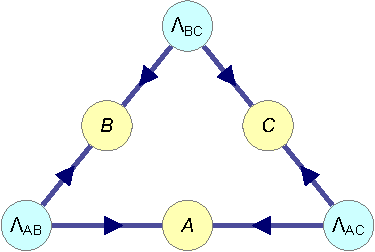
\includegraphics[width=2.5in]{TriDAGcap.pdf}}
\caption{The causal structure of the Triangle scenario, for which the three observed variables lack a common ancestor.}
 \label{fig:TriDAG}
\end{figure}

The Triangle scenario's causal structure dictates that
\begin{align}\begin{split}\label{eq:tristructure}
p&(abc|\lambda_{AB}\lambda_{BC}\lambda_{AC})\\
&=p(a\lambda_{AB}\lambda_{AC})p(b\lambda_{AB}\lambda_{BC})p(c|\lambda_{BC}\lambda_{AC})
\end{split}\end{align}
and accordingly that
\begin{align}\begin{split}\label{eq:triintegration}
&p(abc)=\\
&\sum\limits_{\mathclap{\brackets{\lambda}}}
\begin{pmatrix}p(a|\lambda_{AB}\lambda_{AC})p(b|\lambda_{AB}\lambda_{BC})p(c|\lambda_{BC}\lambda_{AC})\\
\times p(\lambda_{AB})p(\lambda_{BC})p(\lambda_{AC})\end{pmatrix}
\end{split}\end{align}
where the sum is over all three latent variables, i.e. $\brackets{\lambda}={\lambda_{AB},\lambda_{BC},\lambda_{AC}}$.
Once again the first step is to replace each conditional probability with a product sum analogous to \cref{eq:hardytoproductsums}. An example would be 
\begin{align}
p(a|\lambda_{AB}\lambda_{AC})=\sum\limits_{\mathclap{b^{\prime}}}p(a|b^{\prime})p(b^{\prime}|\lambda_{AB}\lambda_{AC})
\end{align}
but we can employ conditional independence relations implied by the causal structure to simplify such terms, namely $p(b^{\prime}|\lambda_{AB}\lambda_{AC})$=$p(b^{\prime}|\lambda_{AB})$ etc. A complete list of allowable substitutions is
\begin{align}%\begin{split}\label[eqs]{eq:triproductsums}
&p(a|\lambda_{AB}\lambda_{AC})=\sum\limits_{\mathclap{b^{\prime}}}p(a|b^{\prime})p(b^{\prime}|\lambda_{AB}),\label{eq:trisplitAtoB}\\
&p(a|\lambda_{AB}\lambda_{AC})=\sum\limits_{\mathclap{c^{\prime}}}p(a|c^{\prime})p(c^{\prime}|\lambda_{AC}),\label{eq:trisplitAtoC}\\
&p(b|\lambda_{AB}\lambda_{BC})=\sum\limits_{\mathclap{a^{\prime}}}p(b|a^{\prime})p(b^{\prime}|\lambda_{AB}),\label{eq:trisplitBtoA}\\
&p(b|\lambda_{AB}\lambda_{BC})=\sum\limits_{\mathclap{c^{\prime}}}p(b|c^{\prime})p(c^{\prime}|\lambda_{BC}),\label{eq:trisplitBtoC}\\
&p(c|\lambda_{BC}\lambda_{AC})=\sum\limits_{\mathclap{a^{\prime}}}p(c|a^{\prime})p(a^{\prime}|\lambda_{AC}),\label{eq:trisplitCtoA}\\
&p(c|\lambda_{BC}\lambda_{AC})=\sum\limits_{\mathclap{b^{\prime}}}p(c|b^{\prime})p(b^{\prime}|\lambda_{BC}).\label{eq:trisplitCtoB}
%\end{split}
\end{align}
%We can simplify \cref{eq:triproductsums} by employing conditional independence relations implied by the causal structure, namely $p(b^{\prime}|\lambda_{AB}\lambda_{AC})$=$p(b^{\prime}|\lambda_{AB})$ etc. So
There are five ways to select equalities from \crefrange{eq:trisplitAtoB}{eq:trisplitCtoB} for substitution into \cref{eq:triintegration} to yield novel compatibility criteria. For the sake of example, let's select \cref{eq:trisplitAtoB,eq:trisplitBtoC,eq:trisplitCtoA}. This yields
\begin{widetext}
\begin{align}\begin{split}\label{eq:triexampleint}
&p(abc)=\sum\limits_{\mathclap{\lambda_{AB},\lambda_{BC},\lambda_{AC},a^{\prime},b^{\prime},c^{\prime}}}
p(a|b^{\prime})p(b^{\prime}|\lambda_{AB})p(b|c^{\prime})p(c^{\prime}|\lambda_{BC})p(c|a^{\prime})p(a^{\prime}|\lambda_{AC})p(\lambda_{AB})p(\lambda_{BC})p(\lambda_{AC})\\
&=
\left(\sum\limits_{\mathclap{b^{\prime}}}\sum\limits_{\mathclap{\lambda_{AB}}}
p(a|b^{\prime})p(b^{\prime}|\lambda_{AB})p(\lambda_{AB})
\right)
\left(\sum\limits_{\mathclap{c^{\prime}}}\sum\limits_{\mathclap{\lambda_{BC}}}
p(b|c^{\prime})p(c^{\prime}|\lambda_{BC})p(\lambda_{BC})
\right)
\left(\sum\limits_{\mathclap{a^{\prime}}}\sum\limits_{\mathclap{\lambda_{AC}}}
p(c|a^{\prime})p(a^{\prime}|\lambda_{AC})p(\lambda_{AC})
\right)\\
&=
\left(\sum\limits_{\mathclap{b^{\prime}}}
p(a|b^{\prime})p(b^{\prime})
\right)
\left(\sum\limits_{\mathclap{c^{\prime}}}
p(b|c^{\prime})p(c^{\prime})
\right)
\left(\sum\limits_{\mathclap{a^{\prime}}}
p(c|a^{\prime})p(a^{\prime})
\right)
%\\&=p(a|b^{\prime})p(b^{\prime})p(b|c^{\prime})p(c^{\prime})p(c|a^{\prime})p(a^{\prime})
\end{split}\end{align}
\end{widetext}
which, being an equality on the observable probabilities, is an exceptionally strict necessary compatibility criterion.
\begin{proposition}\label{prop:TriNoGoNEW}The Triangle causal structure (\cref{fig:TriDAG}) implies that $p(abc)$
\begin{align*}
%&p(abc)\\
&=\!\left(\sum\limits_{\mathclap{b^{\prime}}}
p(a|b^{\prime})p(b^{\prime})
\!\right)\!\!\left(\sum\limits_{\mathclap{c^{\prime}}}
p(b|c^{\prime})p(c^{\prime})
\!\right)\!\!
\left(\sum\limits_{\mathclap{a^{\prime}}}
p(c|a^{\prime})p(a^{\prime})
\!\right)\\
&=\!\left(\sum\limits_{\mathclap{c^{\prime}}}
p(a|c^{\prime})p(c^{\prime})
\!\right)\!\!\left(\sum\limits_{\mathclap{a^{\prime}}}
p(b|a^{\prime})p(a^{\prime})
\!\right)\!\!
\left(\sum\limits_{\mathclap{b^{\prime}}}
p(c|b^{\prime})p(b^{\prime})
\!\right)\\
&=p(c)\sum\limits_{\mathclap{a^{\prime},b^{\prime}}}
p(a|b^{\prime})p(b|a^{\prime})p(a^{\prime}b^{\prime})\\
&=p(a)\sum\limits_{\mathclap{b^{\prime},c^{\prime}}}
p(b|c^{\prime})p(c|b^{\prime})p(b^{\prime}c^{\prime})\\
&=p(b)(\sum\limits_{\mathclap{a^{\prime},c^{\prime}}}
p(a|c^{\prime})p(c|a^{\prime})p(a^{\prime}c^{\prime})
\end{align*}
\end{proposition}
where the additionally equalities come from choosing different identities from \crefrange{eq:trisplitAtoB}{eq:trisplitCtoB} for substitution into \cref{eq:triintegration}, such as the triple of \cref{eq:trisplitAtoC,eq:trisplitBtoA,eq:trisplitCtoB} or the pair of \cref{eq:trisplitAtoB,eq:trisplitBtoA}, etc.
Of course, Prop.~\ref{prop:TriNoGoNEW} can also be weakened by considering individual terms from the sums. Thus
\begin{corollary}\label{cor:TriNoGoNEW}The Triangle causal structure (\cref{fig:TriDAG}) implies that for any ${a^{\prime},b^{\prime},c^{\prime}}$ we have %$p(abc)$
\begin{align*}
%\forall_{a^{\prime}b^{\prime}c^{\prime}}\!:\;
&p(abc) \geq p(a|b^{\prime})p(b^{\prime})p(b|c^{\prime})p(c^{\prime})p(c|a^{\prime})p(a^{\prime})\\
&p(abc) \geq p(a|c^{\prime})p(c^{\prime})p(b|a^{\prime})p(a^{\prime})p(c|b^{\prime})p(b^{\prime})\\
&p(abc) \geq p(c)p(a|b^{\prime})p(b|a^{\prime})p(a^{\prime}b^{\prime})\\
&p(abc) \geq p(a)p(b|c^{\prime})p(c|b^{\prime})p(b^{\prime}c^{\prime})\\
&p(abc) \geq p(b)p(a|c^{\prime})p(c|a^{\prime})p(a^{\prime}c^{\prime})
\end{align*}
\end{corollary}

Consider the following special case, where ${p(A\mathopen{=}0|B\mathopen{=}1)}={p(C\mathopen{=}0|B\mathopen{=}1)}={p(A\mathopen{=}0|C\mathopen{=}1)}=1$. For this case, taking ${a\mathopen{=}b\mathopen{=}c\mathopen{=}1}$ and ${a^{\prime}\mathopen{=}b^{\prime}\mathopen{=}c^{\prime}\mathopen{=}0}$, then the first inequality in Corr.~\ref{cor:TriNoGoNEW} implies $p(A\mathopen{=}B\mathopen{=}C\mathopen{=}1)\geq p(A\mathopen{=}0)p(C\mathopen{=}0)p(C\mathopen{=}0)$.
An example of a probability distribution which is rejected by this special case of Corr.~\ref{cor:TriNoGoNEW} is the W-distribution, 
\begin{align}\label{eq:wdist}
p(abc)=\begin{cases}\nicefrac{1}{3}&\text{if }\; a+b+c=1 \\ 0&\text{otherwise}\end{cases}
\end{align}
where $a,b,c\in\brackets{0,1}$. The W-distribution states that the in any event in which $A,B,C$ are observed, precisely one of them will be found to equal $1$ while the other two will equal $0$. The identity of the variable which takes the value $1$ is uniformly random. 

%Not all choice of substitution from \crefrange{eq:trisplitAtoB}{eq:trisplitCtoB} result in an equality.





\section{Failure of Entropic Inequalities}

It is interesting to note that entropic inequalities \cite{fritz2013marginal,chaves2014novel} fail to recognize the PR-box per \cref{eq:PRbox} as incompatible with the Bell scenario and also the W-type distribution per \cref{eq:wdist} as incompatible with the Triangle scenario, whereas our alternative reasoning is capable of doing so. To reiterate from the abstract, enumeration of entropic inequalities is considered state-of-the-art derivation of necessary albeit insufficient causal structure compatibility criteria \cite{pusey2014gdag}. The insufficiency is a pressing concern in quantum information theory as there are uniquely-quantum distributions which cannot be certified as non-classical by means of entropic inequalities \cite{fritz2012bell}. 

The entropic inequalities associated with the Bell scenario are given by
\begin{align}\begin{split}\label{eq:entropicCHSH}
&H\!\left(A_1,B_1\right)+H\!\left(A_0\right)+H\!\left(B_0\right)
\\&\quad\leq H\!\left(A_0,B_0\right)+H\!\left(A_0,B_1\right)+H\!\left(A_1,B_0\right)
\end{split}\end{align}
and its permutations \cite{chaves2014novel,chaves2012entropic}.

The entropic inequalities associated with the Triangle scenario are given by 
\begin{align}\label{eq:entropicineqs}
\nonumber &I\!\left(A:B\right)+I\!\left(A:C\right)\leq H\!\left(A\right) \\
\nonumber \text{and }\quad&I\!\left(A:B\right)+I\!\left(A:C\right)+I\!\left(B:C\right)\\
&\quad \leq H\!\left(A,B\right)-I\!\left(A:B:C\right)\\
\nonumber \text{and }\quad & I\!\left(A:B\right)+I\!\left(A:C\right)+I\!\left(B:C\right)\\
\nonumber &\quad \leq\frac{H\!\left(A\right)+H\!\left(B\right)+H\!\left(C\right)}{2}-I\!\left(A:B:C\right)
\end{align}
and their permutations \cite{chaves2014novel,Chaves2015infoquantum,pusey2014gdag}.

Note that bipartite mutual information may be understood as $I\!\left(A:B\right)\equiv H\!\left(A\right)+H\!\left(B\right)-H\!\left(A,B\right)$ and tripartite mutual information is defined as $I\!\left(A:B:C\right)\equiv H\!\left(A\right)+H\!\left(B\right)+H\!\left(C\right)-H\!\left(A,B\right)-H\!\left(A,C\right)-H\!\left(B,C\right)+H\!\left(A,B,C\right)$. It is straightforward to demonstrate the the distributions given in \cref{eq:PRbox,eq:wdist} satisfy  \cref{eq:entropicCHSH,eq:entropicineqs} respectively.



\begin{acknowledgments}
\bigskip\noindent\textbf{Acknowledgments}
Research at Perimeter Institute is supported by the Government of Canada through Industry Canada and by the Province of Ontario through the Ministry of Economic Development and Innovation.
\end{acknowledgments}

\nocite{*}
\setlength{\bibsep}{\smallskipamount}
\bibliographystyle{apsrev4-1}
%nocite{apsrev41Control}
\bibliography{apsrevcontrol,hardyinference}



\end{document}